\normaltrue \difficilefalse \tdifficilefalse
\correctionfalse

%\UPSTIidClasse{11} % 11 sup, 12 spé
%\newcommand{\UPSTIidClasse}{12}

\subsection*{Taurus $\star$ \label{C2:06:94}}
\marginnote{\textit{CCINP -- TSI -- 2022.}}
\marginnote{\UPSTIcompetence[2]{C2-06}}
\marginnote{\UPSTIcompetence[2]{A3-05}}
\setcounter{question}{0}

\index{Compétence C2-06}
\index{Taurus}

\index{Train d'engrenages simple}
\ifcorrection
\else
\marginnote{\textbf{Pas de corrigé pour cet exercice.}}
\fi

\ifprof
\else

\begin{marginfigure}
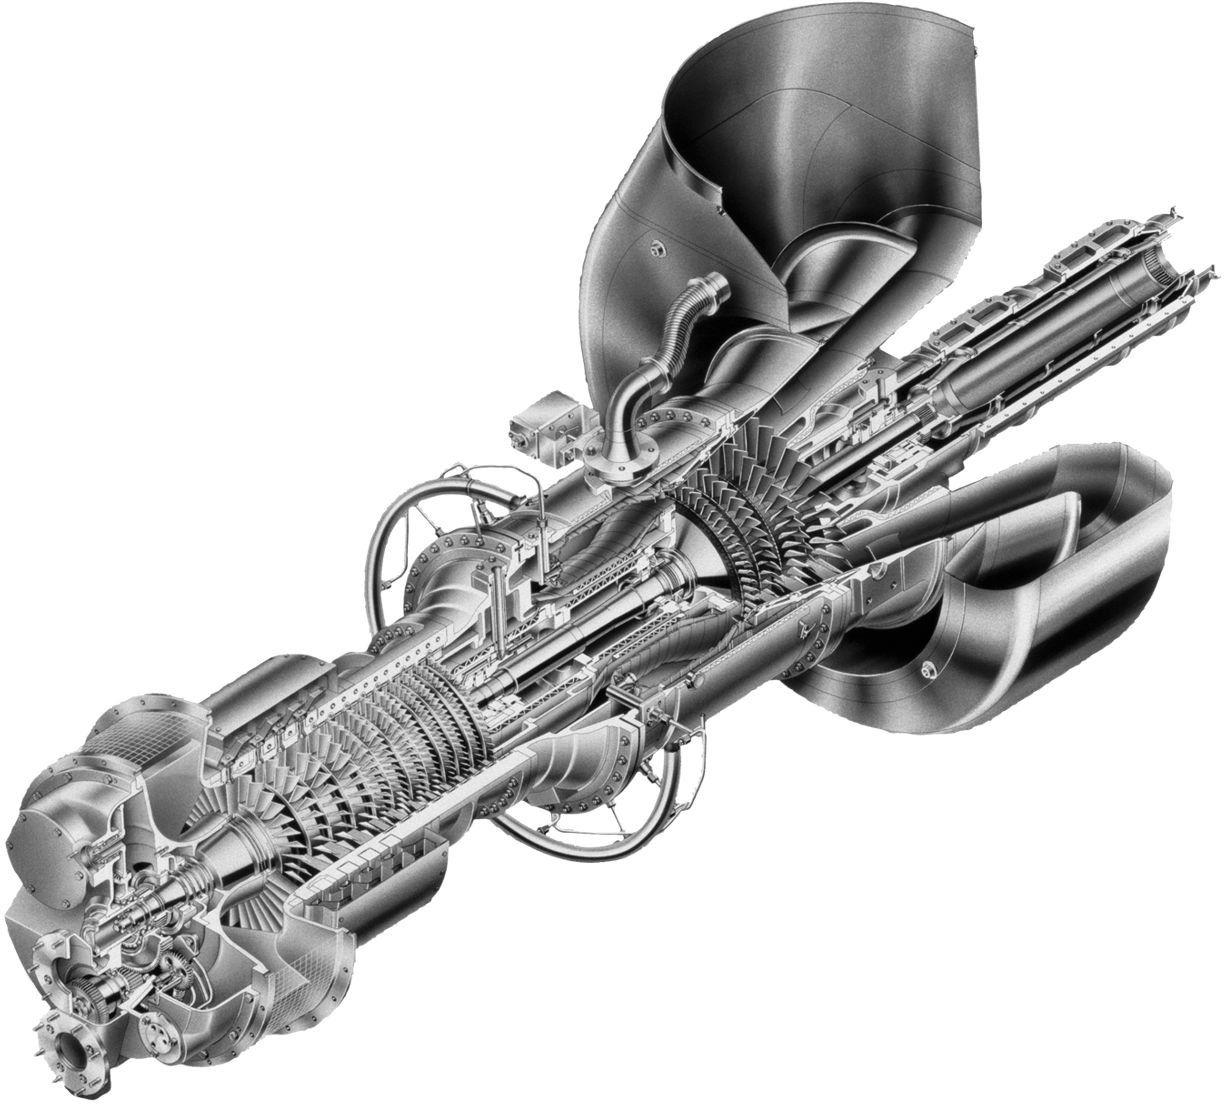
\includegraphics[width=\linewidth]{94_01}
\end{marginfigure}
Pour déterminer le couple au démarrage, il est nécessaire de déterminer le moment d’inertie de
 l’ensemble en rotation ramené sur l’arbre du moteur asynchrone.
 En fonctionnement normal, le schéma cinématique de l’installation retenue est donné figure \ref{fig_94_02}.
 

\begin{figure}[!h]
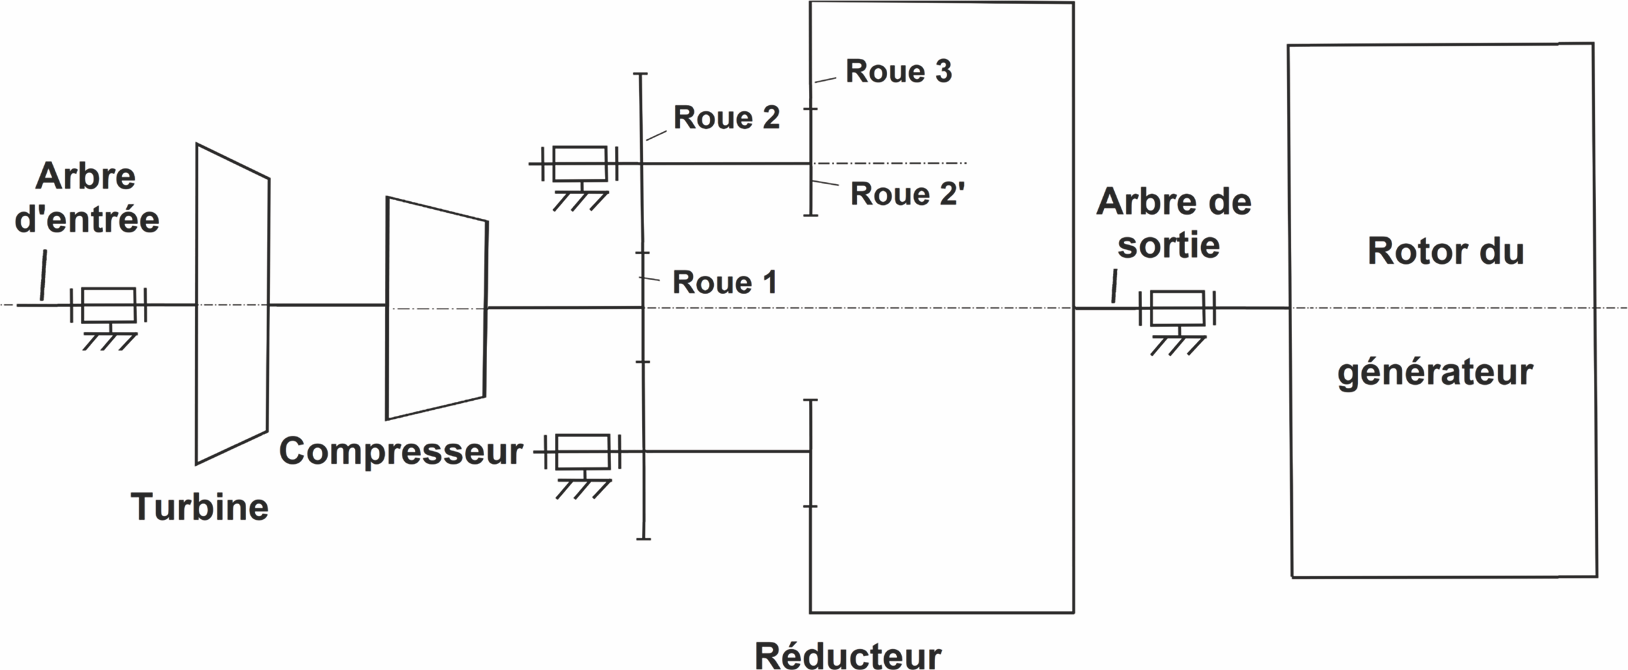
\includegraphics[width=\linewidth]{94_02}
\caption{Schéma cinématique de la turbine à gaz sans démarreur \label{fig_94_02}}
\end{figure}

On donne dans le tableau \ref{tab_94_01} les différents moment d'inertie des éléments composants le système.


\begin{table}[!h]
\begin{tabular}{ll}
\hline
Éléments & Moments d’inertie \\ \hline
 Turbine 	& $J_1= \SI{3,5}{kg.m^2}$ \\
 Compresseur 	& $J_2=\SI{3,4}{kg.m^2}$\\
 Réducteur (ramené sur l’arbre de sortie)&  $J_3=\SI{12,6}{kg.m^2}$\\
 Générateur 	& $J_4=\SI{217,2}{kg.m^2}$\\
 \hline
\end{tabular}
\caption{Moments d’inertie des différents éléments \label{tab_94_01}}
 \end{table}

 Le nombre de dents des différents éléments composant le réducteur est donné dans le tableau \ref{tab_94_02}.

\begin{table}[!h]
\begin{tabular}{llll}
\hline
Roue & Nombre de dents & Roue & Nombre de dents\\ \hline
Roue 1 		& $Z_1 = 40$ 	& Roue 2' 	& $Z_2' = 30$ 	\\
Roue 2 		& $Z_2 = 100$ 	& Roue 3	& $Z_3 = 120$ 	\\
 \hline
\end{tabular}
\caption{Moments d’inertie des différents éléments \label{tab_94_02}}
 \end{table}

 On note $r$ le rapport de réduction entre l’arbre d’entrée et l’arbre de sortie, tel que $r = \dfrac{\omega_{s/0}}{\omega_{e/0}}$ avec :
\begin{itemize}
 	\item  $\omega_{s/0}$ la vitesse de rotation de l’arbre de sortie par rapport au bâti (le support 0);
 	\item $\omega_{e/0}$ la vitesse de rotation de l’arbre d'entrée par rapport au bâti.
\end{itemize}

\fi


\question{En utilisant le schéma cinématique et les données sur les roues, déterminer l’expression littérale du rapport de réduction $r$. Faire ensuite l’application numérique.}
\ifprof
\begin{corrige}
On a $r = \dfrac{\omega_{s/0}}{\omega_{e/0}} = - \dfrac{Z_1 Z_2'}{Z_2 Z_3} $.

\textit{AN :} $r =  - \dfrac{40 \times 30}{100 \times 120}  = -0,1$.
\end{corrige}

\else
\fi

On considère l’ensemble $\Sigma =\{\text{Turbine}, \text{Compresseur}, \text{Réducteur}, \text{Générateur}\}$.

\question{Déterminer l’énergie cinétique de $\Sigma$ par rapport au référentiel galiléen lié au bâti : $\ec{\Sigma}{0}$ en fonction de la vitesse de rotation $\omega_{e/0}$ et des différents moments d’inertie. En déduire l’expression de l’inertie équivalente $\indice{J}{eq}$ ramenée sur l’arbre d’entrée.
 Faire l’application numérique.}
\ifprof 
\begin{corrige}
$\ec{\Sigma}{0} = \dfrac{1}{2}\left( J_1 + J_2 \right) \omega_{e/0}^2 + \dfrac{1}{2}\left( J_3 + J_4 \right) \omega_{e/0}^2r^2 $
$= \dfrac{1}{2}\left(  J_1 + J_2  + \left( J_3 + J_4 \right)r^2  \right)\omega_{e/0}^2$

Et donc $\indice{J}{eq}= J_1 + J_2  + \left( J_3 + J_4 \right)r^2 $.
\end{corrige}
\else
\fi




Le rotor du moteur asynchrone de démarrage dont le moment d’inertie est $J_5=\SI{0,7}{kg.m^2}$ entraîne
 l’ensemble $\Sigma$ par l’intermédiaire du multiplicateur (figure \ref{fig_94_03}). Celui-ci possède un rapport de multiplication $k=6$ et un moment d’inertie négligeable.
 
 \begin{figure}[!h]
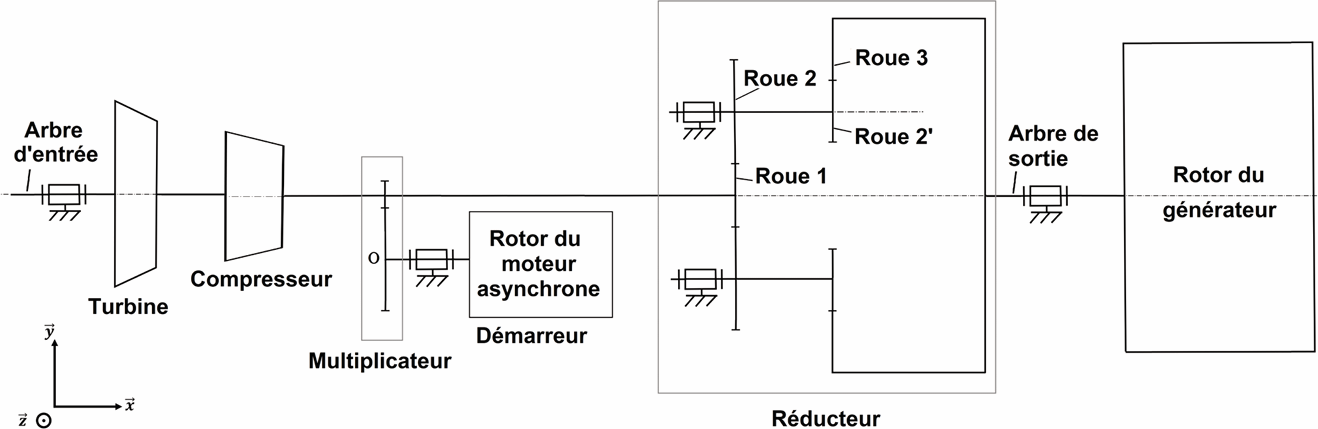
\includegraphics[width=\linewidth]{94_03}
\caption{Schéma cinématique de la turbine à gaz avec démarreur \label{fig_94_03}}
\end{figure}

On considère alors le système $\Sigma' = \{ \Sigma, \text{Moteur asynchrone}, \text{Multiplicateur}\}$.
 
\question{Déterminer l’expression littérale de l’inertie équivalente $\indice{J'}{eq}$ de l’ensemble $\Sigma `$  ramenée sur l’arbre du moteur asynchrone. Faire l’application numérique.}
\ifprof 
\begin{corrige}
On a $\omega_{e/0} = k \omega_{mas/0}$

$\ec{\Sigma'}{0} = \dfrac{1}{2}\indice{J}{eq} \omega_{e/0}^2 + J_5 \omega_{mas/0}^2$
$=\dfrac{1}{2}\left(\indice{J}{eq} k^2 + J_5\right) \omega_{mas/0}^2$.
\end{corrige}
\else
\fi

 

\ifprof
\else
\begin{flushright}
\footnotesize{Corrigé  voir \ref{C2:06:94}.}
\end{flushright}%
\fi